\documentclass{article}

% ----------------------------------- %
%               Packages              %
% ----------------------------------- %

\usepackage[utf8]{inputenc}
\usepackage[english]{babel}
\usepackage{hyperref}
\usepackage{amsmath}
\usepackage{amssymb}
\usepackage{graphicx}
\usepackage{subcaption}
\usepackage{booktabs}
\usepackage[ruled,vlined,linesnumbered]{algorithm2e}
\usepackage[square,numbers]{natbib}
\usepackage[]{algorithm2e}
\usepackage{fancyvrb}
\bibliographystyle{abbrvnat}

% ----------------------------------- %
%               Commands              %
% ----------------------------------- %

\DeclareMathOperator*{\argmax}{argmax}
\DeclareMathOperator*{\argmin}{argmin}

% Bandit Algorithm

\def\numberArm{k}
\def\numberStep{T}
\def\step{t}

\def\reward{r}
\def\rewardNumber{N}
\def\rewardRandom{R}
\def\rewardMean{\mu}
\def\rewardPredMean{\hat{\rewardMean}}
\def\rewardStd{\sigma}

\def\regret{\textbf{r}}

\def\UCB{\text{UCB}}
\def\C{\text{UCB}}
\def\confidenceUCB#1#2{\sqrt{\frac{2\log(#1)}{\rewardNumber_{#2}}}}

% Reinforcement Learning

\def\action{a}
\def\actionSet{\boldsymbol{\mathcal{A}}}
\def\actionEl{\mathcal{A}}
\def\state{s}

\def\rewardSeq{\boldsymbol{R}}
\def\discount{\gamma}

\def\QFun{Q}
\def\QTable{\boldsymbol{\QFun}}
\def\QOptiFun{Q^*}
\def\QNetFun{Q_{\theta}}
\def\QNetFunDash{Q_{\theta'}}

\def\policy{\pi}

\def\gridNumber{N}

\def\upAction{\texttt{UP}}
\def\downAction{\texttt{DOWN}}
\def\leftAction{\texttt{LEFT}}
\def\rightAction{\texttt{RIGHT}}

\def\nothingBlock{\texttt{.}}
\def\agentBlock{\texttt{A}}
\def\wardrobeBlock{\texttt{W}}
\def\poisonBlock{\texttt{P}}
\def\treasureBlock{\texttt{T}}

% ----------------------------------- %
%                 Title               %
% ----------------------------------- %

\title{The CELAR Radio Link Frequency Assignment Problems}
\author{Paul Viallard\\
	\texttt{\href{mailto:paul.viallard@etu.univ-st-etienne.fr}{paul.viallard@etu.univ-st-etienne.fr}} 
	\\\\ Omar Elsabrout\\
	\texttt{\href{mailto:omar.elsabrout@etu.univ-st-etienne.fr}{omar.elsabrout@etu.univ-st-etienne.fr}}}
\date{2 January 2019}

% ----------------------------------- %
%               Document              %
% ----------------------------------- %

\begin{document}
	\maketitle
	
	\begin{abstract}
		As the technical problems grow with time to be more difficult and sophisticated to solve, researchers thrive to explore new solution techniques to solve those problems and export them into real-life applications. Our scope is on huge constrained problems and the usage of multi-agent systems to solve them. Our consideration of multi agents is due to the fact of extremely big number of variables constraints involved in these problems. In our experimental project, we utilize FRODO\cite{FRODO} an open-source framework for distributed constraint optimization. The purpose of our project is to understand the inner workings of distributed constraint solving algorithms and report the best possible solutions we reach for the CLEAR, Centre d’Électronique de l’Armement, radio link frequency assignment.
	\end{abstract}
	
	\section{Introduction}
	As a practical application to our understanding of distributed constraint problem solving, we aim to solve The CLEAR radio link frequency assignment problems made available in the framework of the European project EUCLID CALMA (Combinatorial Algorithms for Military Applications) build from a real network with simplified data. It contains benchmarks of current solvers in order to evaluate our work and grow the community in general.
	
	To go further into details, the cordiality of our constraints is always two, meaning that all of our constraints are binary and do not involve more than two variables. Those variables are non-linear and have finite domains. Moreover, these provided problems are real-world size problems. To draw the picture, the largest of them are composed of around one thousand variables and almost five thousand constraints.
	
	In our report, we provide a description of the problems and data in hand, our approach to model the problems and prepare the data for the FRODO solver, our configuration of FRODO and the reasons behind them and finally results and our analysis of the experiment. All source code of Python scripts and XML files are available for further testing.
	
	\section{Problem Description}
	Explicitly, the radio link frequency assignment problem tackles the task of giving different frequencies to radio data links in pairs to avoid interference. Each radio link is represented by a variable whose domain is the set of all frequencies that are available for this link. 
	
	The essential constraints involve two variables $F_1$ and $F_2$:\[|F_1 - F_2| > K_{12}\] 
	As described in the problem's documentation, the two variables represent two radio links which are close to each other and it may cause an interference. Naturally, the constant $K_{12}$ depends on the position of the two links and also on the physical environment. It is obtained using a mathematical model of electromagnetic waves propagation which is out of the scope of our work. We are more interested in solving the problems than interested in the actual physical details (as long as they do not contribute in our results).
	
	In addition, for each two radio links, two frequencies must be assigned in a way that one is for the communications from A to B and the other is for the communications from B to A. In the case of the CELAR instances, a technological constraint appears which states that the distance in frequency from A to B and from B to A must be exactly equal to 238.
	
	\subsection{Criteria Optimization}
	\label{criteria}
	In order to evaluate the obtained frequency assignments, we need standards upon which we build our judgment of this obtained solution. In the scope of our project, we focus on two main criteria. First, minimization of frequency values. In other words, the frequencies assigned to data links must be minimized for related engineering power consumption concerns. The second criterion is minimizing the number of used frequencies as there will be data links far from each other so they can use the same frequencies. This facilitates installing future data links with the same domains of frequencies.
	
	\subsection{Provided Information}
	For each problem instance, we are provided by domains, variables, constraints and criteria all in separate text files. These files together describe the details of the problem. However, the domain file specifies the numerical values for the available domains to which variables can be assigned to. Moreover, variable files assign them to the aforementioned domains. Next, constraint files involve variables using their number from the variable files. Lastly, criteria files explain the cost of soft constraints (if any) as guidance towards the best feasible solver. All further details of syntax are available in the documentation of CLEAR.
	
	\section{Modeling}
	When it comes to modeling, we discuss two different parts regarding transforming the problems fro the provided format into another format fit for FRODO. The first part is our objective functions regarding cost assignment for constraints to abide the two target criteria previously mentioned in subsection \ref{criteria}. On the other hand, the second part discusses the relation between the number of agents and variables whether it can be optimized or it is not worthy of our computation resources.
	\subsection{Objective Cost Functions}
	We propose our own objective functions to replace the essential constraints introduced by the CLEAR problem itself. The goal behind this move is to customize the resulting cost out of each constraint to achieve minimization of frequency values and minimizing also the number of used frequencies. Furthermore, we also alter the concept of hard constraints in our problems to be completely formed of only soft constraints with an extremely high cost. The reason behind this decision is that it makes the development part easier to debug, it gives a clearer analysis of the performance of the objective function and lastly it leads the investigation to know whether we can reach a fairly expensive solution if the problem is unfeasible or not.
	
	Our first objective cost function targets the minimization of number of frequencies as the formula:
	\[if(|F_1 - F_2| \geq K_{12}), \text{then return 0}, \text{else return } a_t\]
	$a_t$ here corresponds to a vector $a$ that has 5 costs starting with the cost of a hard constraint then the 4 costs provided for soft constraints in descending order. It is represented in an example as the following:
	\begin{align}
		a_0 &= 10000 &\text{ hard}\\
		a_1 &= 1000 &\text{ soft}\\
		a_2 &= 100 &\text{ soft}\\
		a_3 &= 10 &\text{ soft}\\
		a_4 &= 1 &\text{ soft}
	\end{align}
	On the other hand, our second objective cost function tackles the minimization of frequency values as the formula:
	\[a_t||F_1 - F_2| - K_{12}|\]
	Such formula follows the same notation as the previous one with the modification that involves the values of $F_1$, $F_2$ and $K_{12}$ into the return value of the total cost. Both formulas are used for all the tested problems with different resulting solutions.
	\subsection{Agents and Variables}
	Our default strategy for choosing the number of agents is to assign it the same as the number of variables involved in each problem. With this being decided, we aim to have each agent in charge of each link, or in this context a broadcasting tower, as it leaves the problem simply modeled and realistically applicable. Without a doubt, we can change the strategy with another for more optimization. However, it would require more knowledge of the nature of frequencies and the basis upon which the constraints are formed. Due to the huge number of constraints and variables presented in each problem, optimizing the strategy requires a heavier study and considered out of the scope of our interest in the behavior of our solver. 
	
	\section{Parser}
	Our implementation of a parser tool to read the problem's text files is built in a Python 3.6 environment. We utilize a Python based library named LXML\cite{lxml} to construct XML files representing the input problems for FRODO. The parser reads the files \texttt{var.txt}, \texttt{dom.txt}, \texttt{ctr.txt} and \texttt{cst.txt} for each provided instance corresponding to the variable names, used numerical domains, constraints applied on variables and preferred cost per constraint respectively. With the exception of instances 1, 2 and 3 of containing only hard constraints, we ignore costs files and modify the previously mentioned formulas accordingly. All further details on the actual format of text files are available in the CLEAR documentation so we do not repeat them in our report to avoid redundancy. Nonetheless, we move on to explain the construction fo our XML files in the format presented in figure \ref{file_format}.
	\begin{figure}
		\centering
		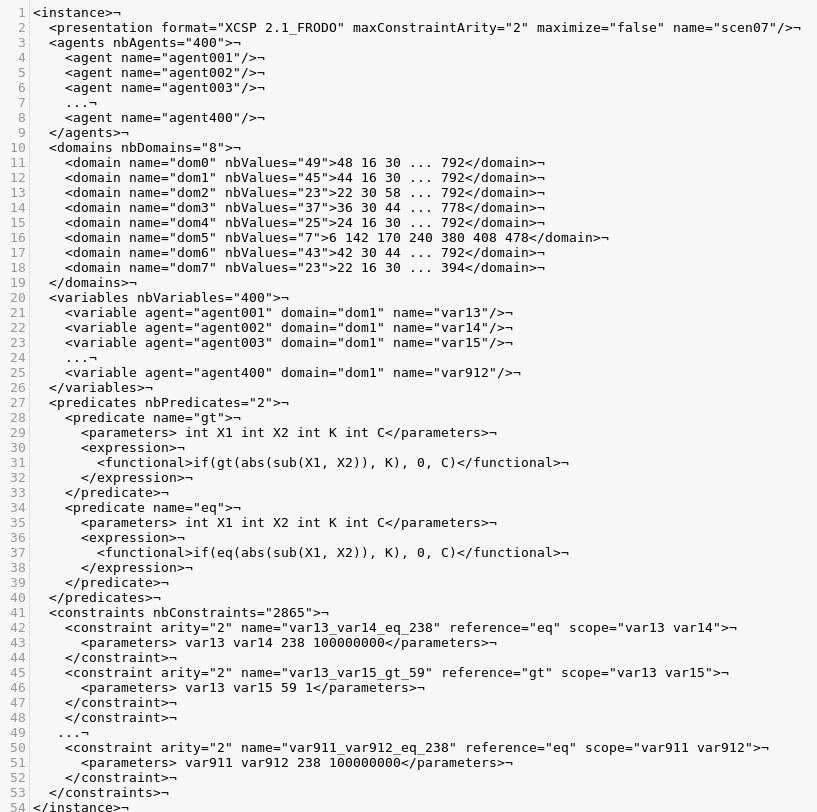
\includegraphics[scale=0.5]{figure/xml.png}
		\caption{A summarized representation of XML file of instance 7.}
		\label{file_format}
	\end{figure}

	For each instance we generate two different XML files for the two objective cost functions. Those two XML files are similar in the parts regarding variables, agents, constraints and domains. On the other hand, they are different when it comes to defining predicates to which the constraints are referenced.
	
	\section{Configuration}
	When it comes to the discussion of the environmental setup of our experiments, we are dictated to define the configuration of our used hardware, used framework and the parameters of such framework. The reason behind the need to explain such configurations is to state the conditions of the experiment to be able to subjectively compare it with other benchmarks.
	
	Our hardware configuration includes an Intel Core i7-8700K processor with 12 cores of 3.7GHz and 24 threads. Such a processor is assumed to be sufficient for the task but it takes long periods to calculate a solution for instances. One other important factor is the available memory which is 64GB of RAM to save the calculated constraints in memory to speed up the search for variable assignments.
	
	While on the other hand, we continue to state our configuration of the FRODO framework. There exist 19 algorithms available to use to solve our problem. However, not all of them have the same performance. Some of them run in exponential time and others are polynomial. Since we have limited hardware resources and instances of problems with huge number of constraints. We decided to use only one polynomial time algorithm which is MGM with two different implemented objective cost functions. The actual detailed comparison of performances among the 19 algorithms can be presented by doing a literature review on their papers which is not the aim of our project since we can never run all algorithms on our hardware. We focus on the performances of our implemented cost functions using MGM. We run the following command to use FRODO:
	
	\texttt{java -cp [frodo.jar path] frodo2.algorithms.AgentFactory [instance XML path] frodo2/agents/MGM/MGMagentJaCoP.xml > [output file path]}
	
	Next, we read the output file with another parser we implemented to save the results and prepare it for plotting and analysis.
	
	\section{Results}
	Finally, we reach the part where we present the output of our experiments. 
	
	
	\begin{tabular}{ |p{3cm}||p{3cm}|p{3cm}|p{3cm}|  }
		\hline
		\multicolumn{4}{|c|}{Country List} \\
		\hline
		Country Name     or Area Name& ISO ALPHA 2 Code &ISO ALPHA 3 Code&ISO numeric Code\\
		\hline
		Afghanistan   & AF    &AFG&   004\\
		Aland Islands&   AX  & ALA   &248\\
		Albania &AL & ALB&  008\\
		Algeria    &DZ & DZA&  012\\
		American Samoa&   AS  & ASM&016\\
		Andorra& AD  & AND   &020\\
		Angola& AO  & AGO&024\\
		\hline
	\end{tabular}
	
	
	
	
	
	
	\begin{figure}
		\centering
		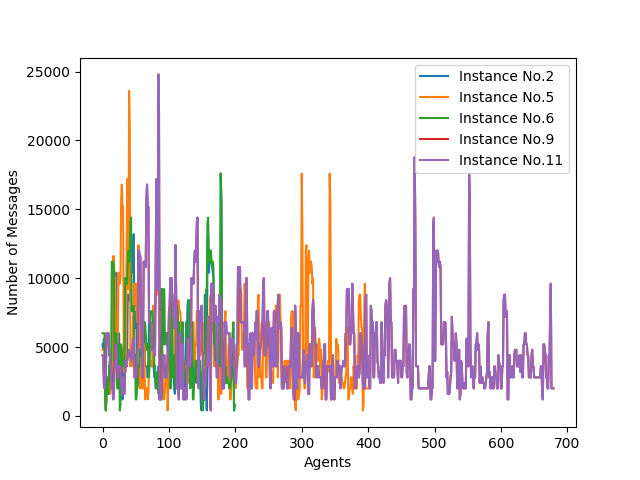
\includegraphics[scale=0.8]{figure/messages.png}
		\caption{A graph showing the number of messages sent and received per agent across the tested problem instances.}
		\label{results:messages}
	\end{figure}
	\section{Conclusion and Perspectives}
	\newpage
	\bibliography{bib.bib}
	
\end{document} 
